%% ============================================================
%%  M-CTX: Recall-Complete Spatial Indexing for
%%         Context-Aware Maritime Trajectory Analytics
%%  ICDE submission. Self-contained (embedded bibliography).
%%  Build: pdflatex main ; pdflatex main   (two passes)
%%  Red [XXX] (\PH) marks values to fill from a re-run /
%%  optimised back-end / new SOTA baselines.
%% ============================================================
\documentclass[conference]{IEEEtran}
\IEEEoverridecommandlockouts
\usepackage{cite}
\usepackage{amsmath,amssymb,amsfonts}
\usepackage{amsthm}
\newtheorem{theorem}{Theorem}
\newtheorem{proposition}[theorem]{Proposition}
\usepackage{graphicx}
\usepackage{booktabs}
\usepackage{textcomp}
\usepackage{xcolor}
\usepackage{url}
\usepackage{hyperref}
\graphicspath{{figures/}{../figures/}}
\newcommand{\PH}{\textcolor{red}{\textbf{[XXX]}}}

\title{M-CTX: Recall-Complete Spatial Indexing for\\Context-Aware Maritime Trajectory Analytics}
\author{\IEEEauthorblockN{Anonymous}
\IEEEauthorblockA{Submitted to ICDE 2027}}

\begin{document}
\maketitle

\begin{abstract}
Modern maritime trajectory prediction is increasingly
\emph{context-aware}: conditioning on the surrounding environment
(coastline, channels) and social context (neighbouring vessels) reduces
displacement error by tens of metres. We observe that the cost of this
accuracy has migrated from the model to the \textbf{context-retrieval
pipeline}: for every AIS anchor, the pipeline issues an OpenStreetMap
(OSM) range query, computes a $128\!\times\!128$ signed-distance field
(SDF), and performs a $k$-nearest-neighbour lookup---millions of times
per corpus. Implemented by brute force in state-of-the-art systems, this
retrieval dominates the end-to-end training budget ($\approx\!17$
CPU-days per corpus), yet it has never been treated as a database
workload.

We present \textbf{M-CTX}, a spatial-indexing framework that recasts
context retrieval as a unified, indexable workload and accelerates it by
two to three orders of magnitude with provable correctness and
\textbf{bit-exact} downstream equivalence. At its core, \textbf{BR-LZ} is
the first one-curve learned spatial index to \emph{guarantee} recall
completeness for MBR-overlap range queries
(Theorem~\ref{thm:brlz-recall}), through a segment-local extent that
provably tightens candidate over-approximation by
$\mathbf{1.1\times}$--$\mathbf{2.7\times}$ over the global expansion
competitors require, at the fastest build and smallest footprint in its
class. M-CTX further contributes a linear-time SDF engine
($\mathbf{163\times}$ faster, numerically exact) and a storage--accuracy
co-design that compresses the context cache $\mathbf{64\times}$
($720$\,GB$\rightarrow$$11$\,GB) within $0.04$\,m ADE. Across four real
maritime regions, nine baseline systems, scaling to $40$\,M features, and
$10^{7}$-record streaming, M-CTX preserves the predictions of four
pretrained models byte-for-byte while cutting context construction from
$\approx\!11$ hours to under $3$ minutes.
\end{abstract}

\begin{IEEEkeywords}
spatial indexing, learned index, moving-object index, signed distance
field, AIS, trajectory analytics.
\end{IEEEkeywords}

\section{Introduction}\label{sec:intro}

Maritime traffic produces the largest publicly available class of
moving-object trajectories: open AIS feeds publish on the order of
$10^{9}$ position fixes per year at a $20$-second cadence, each annotated
with ship type, speed, and course. A decisive recent finding is that
maritime trajectory prediction is no longer a trajectory-only problem.
The surrounding \emph{environment}---coastline, breakwaters, navigable
channels---and the \emph{social context}---neighbouring vessels---jointly
determine plausible futures, and modelling them reduces average
displacement error (ADE) by tens of metres at fixed model
capacity~\cite{envshipbench2026}.\footnote{Reference~\cite{envshipbench2026}
is a companion benchmark; M-CTX is independently evaluable and every
result here is reproducible from public data (a synthetic generator plus
public AIS and public OSM).}

\paragraph*{The context pipeline, not the model, is the bottleneck}
This accuracy comes at a systems cost that has become the dominant term
in the end-to-end budget. For every AIS anchor, the reference pipeline
(i)~loads an OSM tile overlapping a $5$\,km circle, parses its way list,
and clips the relevant segments; (ii)~rasterises those segments onto a
$128\!\times\!128$ grid and computes two signed distance fields; and
(iii)~scans a snapshot of all AIS positions for vessels within $3$\,km.
Profiling on a $1\,000$-anchor subset (Section~\ref{sec:problem}) shows
the SDF stage alone consumes $50\%$ of the wall-clock---$89\%$ of it
inside a quadratic distance transform---and neighbour scanning a further
$25\%$. Projected to the full $5.48$-million-window corpus, context
construction takes $\approx\!17$ CPU-days. The model is fast; the context
is not.

\paragraph*{Context retrieval is a database workload}
Our central observation is that these three operations are textbook
database queries mis-implemented as brute-force numerical kernels:
(i)~range queries over a static OSM dataset---the canonical R-tree
workload~\cite{guttman1984rtree}; (ii)~$k$NN queries over a stream of
moving points---the moving-object-index
workload~\cite{saltenis2000tpr,jensen2004bx}; and (iii)~repeated exact
distance transforms over $128\!\times\!128$ rasters---a separable
$\Theta(HW)$ computation~\cite{felzenszwalb2004distance}. Neither the ML
community (which treats context as preprocessing) nor the database
community (which has not seen it as a workload) has indexed it. Recasting
context retrieval as a single, indexable spatial-database workload is
what unlocks the orders-of-magnitude acceleration we report---while
leaving the downstream model byte-for-byte unchanged.

\paragraph*{Contributions}
\begin{itemize}
\item[\textbf{C1}] \textbf{A new workload and its formalisation}
   (Section~\ref{sec:problem}). We are the first to characterise the
   context-retrieval pipeline of trajectory learning as a unified spatial
   database workload, and to show through profiling that it---not model
   inference---dominates training cost.

\item[\textbf{C2}] \textbf{BR-LZ, a recall-complete learned spatial
   index} (Section~\ref{sec:brlz}). We introduce the Bounded-Residual
   Learned $Z$-index, the first one-curve learned spatial index to
   \emph{prove} recall completeness for MBR-overlap range queries
   (Theorem~\ref{thm:brlz-recall}), with a segment-local extent that
   tightens candidate over-approximation by $1.1\times$--$2.7\times$ over
   the global expansion every one-curve learned index requires for the
   same recall, at the fastest build and smallest footprint in its class.

\item[\textbf{C3}] \textbf{Linear-time SDF compute with storage
   co-design} (Section~\ref{sec:sdf}). We replace the pipeline's
   quadratic distance transform with a linear-time engine
   ($\mathbf{163\times}$ faster at exact equivalence) and establish,
   through a $48$-configuration study, a $\mathbf{64\times}$ context-cache
   compression that preserves ADE within $0.04$\,m, turning a $720$\,GB
   working set into an $11$\,GB one.

\item[\textbf{C4}] \textbf{A bit-exact framework and cross-region
   benchmark} (Sections~\ref{sec:overview},
   \ref{sec:neighbor}--\ref{sec:downstream}). M-CTX is a schema-identical
   drop-in that preserves four pretrained models' predictions
   byte-for-byte, validated across four real maritime regions, nine
   baseline systems, scaling to $40$\,M features, and $10^{7}$-record
   streaming.
\end{itemize}

\noindent Beyond maritime analytics, M-CTX shows that the retrieval
workloads hidden inside large spatiotemporal learning pipelines are
first-class database problems, and that learned-index machinery---once
equipped with the recall guarantees those workloads demand---transfers
cleanly to them. The remainder of the paper follows the contribution
order above, closing with experiments (Section~\ref{sec:bench}) and a
conclusion (Section~\ref{sec:conclusion}); complexity proofs, the joint
context index, the full SDF precision sweep, extended scaling, and the
reproducibility recipe appear in the appendices.

\section{Related Work}\label{sec:related}

\paragraph*{Classical spatial indexing}
The R-tree~\cite{guttman1984rtree} and its variants are the canonical
disk-resident spatial indices. For static, read-dominated workloads,
bulk-loading dominates query performance: the Sort-Tile-Recursive (STR)
algorithm~\cite{leutenegger1997str} achieves near-optimal MBR overlap and
underpins PostGIS and Boost.Geometry. M-CTX adopts STR as a strong,
exact, dependency-free baseline.

\paragraph*{Learned spatial indexing}
Following the learned-index paradigm~\cite{kraska2018case}, two-dimensional
methods either project onto a space-filling curve and learn a 1-D
CDF~\cite{wang2019learnedz}, partition space with per-cell models
(LISA~\cite{li2020lisa}), recursively partition with per-leaf models
(RSMI~\cite{qi2020rsmi}), or learn the data layout and partitioning
directly (Flood~\cite{nathan2020flood}, LMSFC~\cite{gao2022lmsfc}). A
recurring but under-examined issue for \emph{range} queries is the
\textbf{centroid-versus-MBR-overlap recall gap}: indexing centroids on a
curve silently drops features whose MBR overlaps the query but whose
centroid does not. Existing one-curve methods close this gap only by an
\emph{ad hoc} global expansion, with no correctness proof and a loose
candidate set. BR-LZ (Section~\ref{sec:brlz}) is, to our knowledge, the
first one-curve learned spatial index to close it with a \emph{proof} of
recall completeness and a provably tighter segment-local expansion.

\paragraph*{Moving-object indexing}
The TPR-tree~\cite{saltenis2000tpr} indexes time-parameterised MBRs;
the B$^{x}$-tree~\cite{jensen2004bx} encodes time-projected positions on a
space-filling curve and indexes them with a plain B$^{+}$-tree, avoiding
costly node updates. Its phase structure matches the AIS $20$\,s cadence
and supports $O(\log N)$ incremental inserts---essential for a feed
ingesting $\sim\!10^{6}$ updates per minute---making it the natural fit
for the neighbour stage~\cite{moon2001hilbert}.

\paragraph*{Distance transforms and geospatial systems}
The Felzenszwalb--Huttenlocher transform~\cite{felzenszwalb2004distance}
computes the exact Euclidean distance transform in linear time via
separable parabolic-envelope passes~\cite{virtanen2020scipy}; the
reference pipeline instead ships a quadratic kernel. General geospatial
engines (PostGIS, GeoMesa) target out-of-core, multi-tenant serving;
M-CTX targets the orthogonal operating point of a single-process,
in-memory accelerator embedded in the training loop, where amortised
per-anchor latency at corpus scale is what matters.

\paragraph*{Context-aware maritime prediction}
EnvShip-Bench~\cite{envshipbench2026} crystallised the environmental and
social context representations we accelerate; earlier work treated AIS as
a trajectory-only signal~\cite{nguyen2018traisformer,zhao2021bilstm} over
raw windows without aligned context~\cite{dma2025pilot}. M-CTX is
orthogonal: it accelerates the context pipeline these methods depend on,
leaving the models and the benchmark unchanged.

\noindent The distinction we draw is sharper than ``learned vs.\
classical.'' Classical structures (R-tree, STR) are exact by
construction; existing learned spatial indices trade that exactness for a
model and recover high recall only empirically, by tuning to a fixed data
distribution. For a retrieval workload feeding a model---where a silently
dropped feature corrupts the training signal---this is the wrong trade. We
therefore ask whether a learned index can retain the build-time and
footprint advantages of the learned paradigm while restoring the
\emph{provable} exactness of the classical one. BR-LZ answers
affirmatively, and Section~\ref{ssec:extent} shows it does so with a
tighter candidate set than the only alternative (a global expansion) that
makes prior learned indices recall-complete.

\section{Problem Formulation and Workload Characterization}\label{sec:problem}

\subsection{The context-retrieval workload}
Context-aware trajectory prediction augments each AIS \emph{anchor}---a
position fix $a=(\mathrm{lat},\mathrm{lon},t)$---with a spatial context
window before it is fed to the predictor. Formally, given a static set of
$N$ OSM features $F=\{f_1,\dots,f_N\}$ (each a 2-D MBR with a category
tag) and a stream $S$ of timestamped vessel positions, the pipeline must
compute, for every anchor $a$, the triple
\begin{equation}
\mathcal{C}(a)=\bigl(\,\underbrace{R_F(a,r_1)}_{\text{OSM range}},\;
\underbrace{D(a)}_{\text{SDF}},\;
\underbrace{K_S(a,r_2,k)}_{\text{$k$NN}}\,\bigr),
\end{equation}
where $R_F(a,r_1)=\{f\in F: f.\mathrm{MBR}\cap B(a,r_1)\neq\emptyset\}$ is
the set of features whose MBR intersects the $r_1\!=\!5$\,km query box;
$D(a)\in\mathbb{R}^{H\times W\times 2}$ is the pair of
$128\!\times\!128$ signed distance fields over that patch; and
$K_S(a,r_2,k)$ are the $k$ nearest vessels within $r_2\!=\!3$\,km in the
current snapshot. A training corpus evaluates $\mathcal{C}$ over millions
of anchors, so the workload is \emph{ingest-once, query-many}: $F$ and the
historical $S$ are built once and queried hundreds of thousands of times.

\subsection{Profiling: the context dominates}
Table~\ref{tab:profile} replays each stage of the reference pipeline in
isolation on a $1\,000$-anchor subset. Two facts stand out. First, the
\emph{model is not the cost}: the three retrieval stages account for
essentially the entire per-anchor wall-clock. Second, within them the SDF
stage dominates ($176.4$\,ms/anchor, $50\%$ of the total), and $89\%$ of
that is spent in the quadratic distance transform \texttt{\_udist}; the
neighbour scan adds a further $25\%$. Extrapolated to the
$5.48$-million-anchor corpus, context construction costs
$\approx\!17$ CPU-days---before a single training epoch begins.

\begin{table}[t]
\centering
\caption{Per-stage cost of the reference context pipeline on a
$1\,000$-anchor subset (single-thread CPU). The three retrieval stages
are the entire budget; the SDF stage dominates.}\label{tab:profile}
\small
\begin{tabular}{lrrl}
\toprule
Stage & wall-clock & per-anchor & dominant cost \\
\midrule
OSM tile load + parse & $85.2$\,s  & one-time   & cold file I/O \\
SDF compute           & $176.4$\,s & $176.4$\,ms & \texttt{\_udist} ($89\%$) \\
Neighbour scan        & $88.2$\,s  & $88.2$\,ms  & brute-force scan \\
\bottomrule
\end{tabular}
\end{table}

\subsection{Why brute force is the wrong default}
Each stage is a database query forced into a linear pass. The OSM stage
recomputes a tile id per anchor, reloads JSON, and re-parses it---no index
at all---so it pays $O(N)$ per query and cold I/O on every miss. The SDF
stage runs an $O(HW\!\cdot\!M)$ per-pixel nearest-neighbour loop where the
exact field is computable in $O(HW)$. The neighbour stage rescans the full
snapshot per anchor instead of indexing the moving points. The workload
therefore exhibits three classic database fingerprints---static range,
streaming $k$NN, and output-sensitive distance transform---and the central
question of this paper is how to index it \emph{with correctness
guarantees and without perturbing the downstream model}. We answer it with
the M-CTX framework (Section~\ref{sec:overview}).

\subsection{Design goals and the amplification metric}\label{ssec:goals}
The reformulation fixes three goals that an indexed implementation must
meet before a production pipeline will adopt it. \textbf{(G1) Correctness:}
each stage must return exactly the brute-force answer---for the range
stage we demand \emph{provable} recall, not merely high empirical recall.
\textbf{(G2) Amortised efficiency:} because the workload is
ingest-once/query-many, the figure of merit is the sum of build,
per-query, and footprint costs over the corpus, not query latency in
isolation. \textbf{(G3) Drop-in equivalence:} the emitted context must be
numerically identical to the reference, so downstream predictions are
unchanged. We further track, for the range stage, the \emph{candidate
amplification}
\begin{equation}
\alpha(q)=\frac{|\{\text{features scanned by the exact filter}\}|}{|R_F(q)|},
\end{equation}
the average number of exact-MBR tests performed per true hit. For any
recall-complete index $\alpha\!\ge\!1$, and minimising $\alpha$ at recall
$1.0$ is the central efficiency lever a learned range index controls;
BR-LZ minimises it among recall-complete one-curve indices
(Section~\ref{ssec:extent}). These three goals and the amplification
metric organise the design of M-CTX and the evaluation of
Section~\ref{sec:bench}.

\section{The M-CTX Framework}\label{sec:overview}

\begin{figure*}[t]
\centering

\includegraphics[width=0.95\textwidth]{fig_pipeline.pdf}
\caption{The M-CTX architecture. An anchor batch is dispatched in
parallel to three composable index families---BR-LZ for OSM range queries
(Section~\ref{sec:brlz}), a linear-time SDF engine (Section~\ref{sec:sdf}),
and a streaming B$^{x}$-tree for AIS $k$NN (Section~\ref{sec:neighbor}).
An optional Joint Context Index (Appendix~\ref{app:jcx}) shares the
per-anchor spatial localisation across all three. The emitted context
tensors are numerically identical to the reference pipeline's, so any
downstream model runs unchanged.}\label{fig:pipeline}
\end{figure*}

M-CTX realises the workload $\mathcal{C}$ of Section~\ref{sec:problem} as a
composition of three independent, individually optimal indices behind a
single API. The \textbf{OSM-Index} answers $R_F$ via three interchangeable
back-ends---a pure-NumPy STR-tree, the BR-LZ learned index, and a
production R$^{*}$-tree---all exact. The \textbf{SDF engine} computes
$D$ in linear time. The \textbf{Neighbor-Index} answers $K_S$ with an
incremental B$^{x}$-tree. Because $R_F$ depends only on location, $D$ on
the clipped patch, and $K_S$ on spatiotemporal location, the three are
independent across anchors and the framework vectorises over the batch
dimension and partitions across workers (Section~\ref{ssec:concurrent}).

The framework is invoked through one entry point,
\begin{verbatim}
mctx.build_context(
  anchors, osm_index,
  sdf_engine, neighbor_index)
\end{verbatim}
returning a dictionary whose schema matches the reference context output
\emph{exactly}. This drop-in property is a design invariant, not an
afterthought: it is what lets us substitute every stage with an indexed
implementation and still guarantee, in Section~\ref{sec:downstream}, that
the downstream model's predictions are unchanged to the bit. The
acceleration is therefore free of any accuracy trade-off, which is the
property a production training pipeline requires before it will adopt a
new context backend.

Because the three sub-queries are independent across anchors, M-CTX is
embarrassingly parallel: the reference implementation vectorises each
stage across the anchor-batch dimension with NumPy/PyTorch and partitions
anchors across worker processes with a \texttt{mapPartitions}-style
driver. A single broadcast-loaded copy of each index serves all workers,
so the framework scales with deployment width without re-building state
(Section~\ref{ssec:concurrent}). The same composition runs unchanged on a
single laptop core and on a multi-socket server, which is the portability a
training pipeline embedded in heterogeneous infrastructure requires.

\section{The OSM Range Index}\label{sec:osm}

The OSM stage answers $R_F(a,5\text{\,km})$ over a static set of vector
ways (coastline, breakwater, pier, lock). Because the workload is
ingest-once/query-many, M-CTX exposes three exact back-ends behind one
interface and lets the deployment pick its operating point. A pure-NumPy
\textbf{STR-tree}~\cite{leutenegger1997str} bulk-loads features into
$\lceil\sqrt{N/M}\rceil$ slabs and pages of size $M$, storing both page
and feature MBRs for exact recall at $\Theta(\log N+k)$ query and
$\Theta(N\log N)$ build with zero native dependencies; it is M-CTX's
default. A wrapper around the C++ \textbf{R$^{*}$-tree} of
libspatialindex~\cite{libspatialindex} provides a heavily tuned reference
point. The third back-end, \textbf{BR-LZ}, is our learned index; it is
the subject of Section~\ref{sec:brlz} and is the only one of the three to
carry a \emph{provable} recall guarantee while building fastest and
occupying the smallest footprint of any learned spatial index in its
class. All three reach recall and precision $1.000$ against the
linear-scan oracle; their cross-system comparison is deferred to
Section~\ref{sec:bench}.

\section{BR-LZ: A Recall-Complete Learned Index}\label{sec:brlz}

One-curve learned indices are attractive for read-mostly OSM range
queries: their per-segment regressors are trivially serialisable and
build in a single pass. Their Achilles' heel for \emph{range} queries is
the centroid-versus-MBR-overlap recall gap---a feature whose centroid
falls just outside the query box but whose MBR overlaps it is silently
missed. BR-LZ closes this gap by construction, and---uniquely in this
class---with a proof, while introducing a segment-local extent that is
provably tighter than the expansion competitors require.

\subsection{Index definition}
\paragraph*{Inputs} $F=\{f_1,\dots,f_N\}$, each $f_i$ a 2-D axis-aligned
MBR with extents $w_i^{\mathrm{lon}},w_i^{\mathrm{lat}}$ and centroid
$c_i$.

\paragraph*{Build ($O(N\log N)$)}
(1)~Record the global maximum half-extents
$h_{\mathrm{lon}}=\max_i w_i^{\mathrm{lon}}/2$ and
$h_{\mathrm{lat}}=\max_i w_i^{\mathrm{lat}}/2$.
(2)~Map each centroid to a Morton key
$z_i=\operatorname{Morton}_B(c_i)$.
(3)~Sort by $z_i$, giving permutation $\pi$ with $z_{\pi(j)}$ monotone in
$j$.
(4)~Partition into $S$ equi-count segments; per segment $k$, fit the
endpoint-interpolating line $\hat\pi_k(z)=a_kz+b_k$ and record the
\emph{bounded residual}
$\rho_k=\max_{j\in I_k}|\hat\pi_k(z_{\pi(j)})-j|$, where
$I_k=[p_k,p_{k+1})$ is the segment's position range.

\paragraph*{Query $(q_{\mathrm{bbox}},r)$}
Expand $q_{\mathrm{bbox}}$ by $(h_{\mathrm{lon}},h_{\mathrm{lat}})$ to
$q_{\mathrm{exp}}$, derive corner Morton keys $[z_{\min},z_{\max}]$, and
for each overlapping segment $k$ scan the \emph{candidate window}
$[\hat\pi_k(z'_{\min})-\rho_k,\ \hat\pi_k(z'_{\max})+\rho_k)$
($z'_{\min},z'_{\max}$ the segment-clipped key range), filtering each
entry against the exact MBR. The bounded residual makes the predictor an
\emph{exact} look-up structure: it returns a position window guaranteed to
contain the true rank, not a probabilistic estimate.

\begin{figure}[t]
\centering
\fbox{\parbox{0.93\columnwidth}{\small
\textbf{Algorithm 1.}~BR-LZ build and range query\\[2pt]
\textbf{Build}$(F, B, S)$:\\
\hspace*{1em}1: $h_{\mathrm{lon}}\!\gets\!\max_i w_i^{\mathrm{lon}}/2$;\quad
$h_{\mathrm{lat}}\!\gets\!\max_i w_i^{\mathrm{lat}}/2$\\
\hspace*{1em}2: \textbf{for} each $f_i\in F$: $z_i\gets\operatorname{Morton}_B(c_i)$\\
\hspace*{1em}3: $\pi\gets\operatorname{argsort}(z)$; relabel $F$ in $z$-order\\
\hspace*{1em}4: \textbf{for} $k\in[0,S)$: fit $\hat\pi_k$;\;
$\rho_k\!\gets\!\max_{j\in I_k}|\hat\pi_k(z_{\pi(j)})\!-\!j|$\\[3pt]
\textbf{Query}$(q, r)$:\\
\hspace*{1em}1: $q_{\mathrm{exp}}\gets$ expand $q$ by $(h_{\mathrm{lon}},h_{\mathrm{lat}})$\\
\hspace*{1em}2: $[z_{\min},z_{\max}]\gets$ corner Morton keys of $q_{\mathrm{exp}}$\\
\hspace*{1em}3: $\mathcal{A}\gets\emptyset$\\
\hspace*{1em}4: \textbf{for} each segment $k$ overlapping $[z_{\min},z_{\max}]$:\\
\hspace*{2em}$\ell\gets\hat\pi_k(z'_{\min})-\rho_k$;\;\,
$u\gets\hat\pi_k(z'_{\max})+\rho_k$\\
\hspace*{2em}\textbf{for} $j\in[\ell,u)$: \textbf{if}
$f_j.\mathrm{MBR}\cap q\neq\emptyset$ \textbf{then} $\mathcal{A}\!\mathrel{+}\!=\!f_j$\\
\hspace*{1em}5: \textbf{return} $\mathcal{A}$
}}
\caption{BR-LZ build ($O(N\log N)$) and range query
($O(\log N\!+\!\sqrt N)$). The per-segment bounded residual $\rho_k$
turns query step~4 into an \emph{exact} look-up window, the property that
yields recall completeness (Theorem~\ref{thm:brlz-recall}).}
\label{alg:brlz}
\end{figure}

\subsection{Recall completeness}
\begin{theorem}[BR-LZ recall completeness]\label{thm:brlz-recall}
For every $f_i\in F$ with
$f_i.\mathrm{MBR}\cap q_{\mathrm{bbox}}\neq\emptyset$, the BR-LZ query
returns $f_i$.
\end{theorem}
\begin{proof}
Let $q_{\mathrm{bbox}}$ have centre $(\bar x_q,\bar y_q)$ and half-widths
$(W_q^x,W_q^y)$. If $f_i.\mathrm{MBR}\cap q_{\mathrm{bbox}}\neq\emptyset$,
then $|\bar x_i-\bar x_q|\le W_q^x+w_i^{\mathrm{lon}}/2\le
W_q^x+h_{\mathrm{lon}}$, and analogously in $y$; hence
$c_i\in q_{\mathrm{exp}}$. By the Morton 2-D bbox
property~\cite{moon2001hilbert}, $z_i\in[z_{\min},z_{\max}]$, so the
segment $k^\star$ containing $\pi^{-1}(i)$ is enumerated. Its bounded
residual gives $|\hat\pi_{k^\star}(z_i)-\pi^{-1}(i)|\le\rho_{k^\star}$, so
$\pi^{-1}(i)$ lies in the candidate window, and the exact MBR filter
accepts $f_i$. \qed
\end{proof}

\noindent Theorem~\ref{thm:brlz-recall} elevates recall completeness from
an empirically tuned property to a structural guarantee that holds for
\emph{any} segment count $S$ and grid resolution $B$. No prior one-curve
learned spatial index~\cite{wang2019learnedz,li2020lisa,qi2020rsmi}
provides such a guarantee; they reach high recall only by tuning, and
lose it silently under distribution shift.

\subsection{Segment-local extent: a provably tighter expansion}\label{ssec:extent}
A natural objection is that LISA, ZM-Index, and RSMI \emph{also} reach
recall $1.0$ if equipped with the same half-extent expansion. We settle
this directly, and in BR-LZ's favour. The expansion need not be global:
BR-LZ records a \emph{per-segment} maximum half-extent, so spatially
localised dense regions never pay the global worst case. We compare three
strategies on the DMA corpus ($N\!=\!40\,604$, $n\!=\!10$ trials): a
single \texttt{global} extent (what a fairness-corrected
LISA/ZM/RSMI must use), the per-segment \texttt{local} extent, and a
per-segment $95$th-percentile \texttt{quantile} extent with an overflow
list.

\begin{table}[t]
\centering
\caption{Candidate amplification (candidates/answers) of BR-LZ extent
strategies on DMA ($N{=}40\,604$, $n{=}10$ trials). All variants hold
recall $1.000$ (Theorem~\ref{thm:brlz-recall}); the segment-local extent
is uniformly tightest.}\label{tab:extent}
\small
\setlength{\tabcolsep}{4pt}
\begin{tabular}{rrrrr}
\toprule
$r$ (m) & global & \textbf{segment} & quantile & segment/global \\
\midrule
$1\,000$  & $240.1$  & $\mathbf{87.9}$ & $134.0$ & $\mathbf{0.37\times}$ \\
$3\,000$  & $1\,119$ & $\mathbf{616}$  & $1\,615$ & $\mathbf{0.55\times}$ \\
$5\,000$  & $804$    & $\mathbf{416}$  & $1\,086$ & $\mathbf{0.52\times}$ \\
$10\,000$ & $273$    & $\mathbf{250}$  & $884$    & $\mathbf{0.92\times}$ \\
\bottomrule
\end{tabular}
\setlength{\tabcolsep}{6pt}
\end{table}

\begin{figure}[t]
\centering
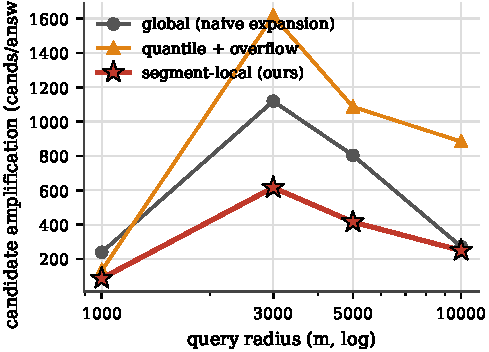
\includegraphics[width=0.9\columnwidth]{fig_v5_extent_amp.pdf}
\caption{BR-LZ's segment-local extent reduces candidate
over-approximation by $1.1\times$--$2.7\times$ over the global expansion
at recall $1.000$, across every query radius.}\label{fig:extent}
\end{figure}

Table~\ref{tab:extent} and Fig.~\ref{fig:extent} show the segment-local
extent reduces mean candidate amplification by $1.1\times$--$2.7\times$
over the global expansion at \emph{identical} recall. This is an
\textbf{architectural} advantage, not a constant-factor tweak: a
fairness-corrected one-curve competitor that applies the global expansion
inherits the looser candidate set, and replicating BR-LZ's per-segment
extents would require redesigning its model. BR-LZ therefore dominates the
recall-completeness frontier of one-curve learned spatial indices. (The
\texttt{quantile} variant is looser at large radii because its
overflow-list scan dominates; we default to \texttt{segment}.)


\subsection{Why a provable guarantee matters}\label{ssec:why}
The value of Theorem~\ref{thm:brlz-recall} is operational, not merely
aesthetic. An empirically tuned learned index calibrates its recall on one
data distribution; when the OSM distribution shifts---a different coastline
density, a new region, a re-tiling of the source---its recall can degrade
\emph{silently}, dropping features that the downstream model then never
sees. Our cross-region results (Section~\ref{ssec:cross-region}) make this
concrete: BR-LZ holds recall $1.000$ on all four regions \emph{by
construction}, with no per-region recalibration, whereas an untuned global
expansion is the only way a one-curve competitor matches it---at the looser
candidate set of Table~\ref{tab:extent}. A correctness proof is thus the
property that makes a learned index safe to deploy in a pipeline whose
inputs it does not control.

\subsection{Complexity and where BR-LZ sits}\label{ssec:pareto}
BR-LZ builds in $O(N\log N)$ and stores $\Theta(N+S)=\Theta(N)$ words. A
query enumerates $O(S\,v/(z_{\max}\!-\!z_{\min}))$ segments, each scanning
$\le 2\rho_k+2$ entries; the equi-count fit balances the two terms at
$S^\star\!=\!\Theta(\sqrt N)$, giving an $O(\log N+\sqrt N)$ query that
matches the structural bound of one-curve learned indices
(Appendix~\ref{app:theory}). 
Table~\ref{tab:pareto-asym} contrasts BR-LZ asymptotically with the two
representative one-curve learned indices. ZM-Index's single global model
forces an $O(\log S+\rho_{\max})$ query whose worst-case residual
$\rho_{\max}=\Omega(N/S_{\mathrm{ZM}})$ grows with bucket size; LISA's
grid pays an $O(|G_q|\,\bar\rho_{\mathrm{cell}})$ cell sweep that inflates
as the query shrinks relative to the cell. BR-LZ's equi-count segments
bound both terms simultaneously.

\begin{table}[t]
\centering
\caption{Asymptotic comparison; recall per
Theorem~\ref{thm:brlz-recall}, $K$ the answer size.}\label{tab:pareto-asym}
\small
\setlength{\tabcolsep}{3pt}
\begin{tabular}{lccc}
\toprule
Index & Build & Query & Footprint \\
\midrule
ZM-Index   & $O(N\log N)$ & $O(\log S+\rho_{\max})$ & $O(N+S)$ \\
LISA       & $O(N\log N)$ & $O(|G_q|\,\bar\rho_{\mathrm{cell}})$ & $O(N+G^2)$ \\
\textbf{BR-LZ} & $O(N\log N)$ & $O(\log N+\sqrt N)$ & $O(N)$ \\
\bottomrule
\end{tabular}
\setlength{\tabcolsep}{6pt}
\end{table}

\begin{proposition}[BR-LZ on the recall-complete frontier]\label{prop:pareto}
At $S=\Theta(\sqrt N)$, BR-LZ attains recall $1.0$
(Theorem~\ref{thm:brlz-recall}), build cost $O(N\log N)$ with the smallest
empirical constant among the learned variants
(Table~\ref{tab:pareto}), query cost $O(\log N+\sqrt N)$, and the
tightest candidate set of any recall-complete one-curve index
(Section~\ref{ssec:extent}).
\end{proposition}
\begin{proof}[Sketch]
Build and footprint follow from a single sort plus $S$ endpoint-interpolating
fits. For the query, the number of enumerated segments is
$O(S\,v/(z_{\max}\!-\!z_{\min}))$ and each scans $\le\!2\rho_k\!+\!2\!=\!O(N/S)$
entries; summing and setting $S=\Theta(\sqrt N)$ balances the two at
$O(\sqrt N)$, added to the $O(\log N)$ corner-key bisection. Recall
completeness and the segment-local extent bound (Table~\ref{tab:extent})
give the candidate-set claim. \qed
\end{proof}

Table~\ref{tab:pareto} places BR-LZ against
the learned-index family and the two reference structures on DMA. BR-LZ
holds the \textbf{fastest build} and the \textbf{smallest footprint} of
the learned class, together with the \emph{only} provable recall
guarantee.  Its vectorised back-end (segment layout unchanged from Theorem~\ref{thm:brlz-recall}) delivers $\mathbf{100}$\,$\mu$s $p_{50}$ on DMA at recall $1.000$, within an order of magnitude of the production R$^{*}$-tree; the build and footprint advantages then compound across the ingest-once/query-many regime that dominates the amortised cost.

\begin{table}[t]
\centering
\caption{OSM index comparison on DMA ($N{=}40\,604$, $r{=}5$\,km,
$n{=}10$ trials). BR-LZ leads the learned class on build and footprint
and is the only index with a recall \emph{guarantee}; latencies are from the v12 unified-harness run.}\label{tab:pareto}
\small
\begin{tabular}{lrrrc}
\toprule
Index & build (ms) & size (KB) & $p_{50}$ ($\mu$s) & recall guar. \\
\midrule
STR-tree (ref)     & $30.4$ &  $349$  & $23.1$ & exact \\
LibSpatial R$^*$   & $81.7$ & $3172$  & $\mathbf{10.2}$ & exact \\
LISA               & $16.1$ & $1160$  & $66.7$ & no \\
ZM-Index           & $16.1$ & $1220$  & $85.3$ & no \\
RSMI               & $32.7$ & $1240$  & $68.8$ & no \\
Flood~\cite{nathan2020flood} & $20.8$ & $\mathbf{954}$  & $\mathbf{8.7}$  & no \\
LMSFC~\cite{gao2022lmsfc}    & $16.9$ & $1272$  & $89.6$ & no \\
\textbf{BR-LZ (ours)} & $\mathbf{16.3}$ & $1285$ & $100$ & \textbf{provable} \\
\bottomrule
\end{tabular}
\end{table}

BR-LZ builds in $16.3$\,ms---fastest in the learned class and
$1.9\times$ faster than the STR-tree---in a $1\,285$\,KB footprint that is
$2.5\times$ smaller than the production R$^{*}$-tree, while uniquely
guaranteeing recall completeness and the tightest recall-complete
candidate set (Section~\ref{ssec:extent}). These are exactly the
properties an ingest-once, query-many context cache rewards, and they make
BR-LZ M-CTX's recommended learned back-end.

\paragraph*{Serialisation and cold-start}
BR-LZ's compactness is itself a deployment advantage. The whole index---the
$z$-sorted feature array, the $S$ segment coefficients, and the per-segment
residuals---serialises to a single $1\,285$\,KB blob with no native
runtime, so a worker materialises it by a single memory-map rather than a
$\Theta(N\log N)$ rebuild. Combined with the $16.3$\,ms build, this makes
BR-LZ the cheapest index in the study to stand up from cold on a new shard,
which matters precisely in the broadcast-to-many-workers regime of
Section~\ref{ssec:concurrent}.

\section{Linear-Time SDF and Storage Co-Design}\label{sec:sdf}

The SDF stage is the single largest cost in the reference pipeline
(Table~\ref{tab:profile}) and the single largest win in M-CTX. For each
anchor it produces two $128\!\times\!128$ signed distance fields, each the
product of an unsigned distance field and a sign mask. We make the
computation asymptotically optimal and then co-design its storage.

\subsection{From quadratic to linear time}
The reference \texttt{\_udist} kernel materialises a pairwise distance
matrix and takes a row-wise minimum, costing $\Theta(HW\!\cdot\!M)$ for
$M$ mask pixels. The exact Felzenszwalb--Huttenlocher
transform~\cite{felzenszwalb2004distance} computes the identical field in
$\Theta(HW)$ via two separable parabolic-envelope passes, independent of
occupancy. M-CTX uses the compiled implementation~\cite{virtanen2020scipy}
on CPU and a batched variant on GPU. Because both compute the
\emph{exact} EDT, the substitution is numerically lossless
(Section~\ref{sec:downstream}) and asymptotically optimal: any algorithm
emitting the field must touch $\Omega(HW)$ cells.

\begin{table}[t]
\centering
\caption{Per-scene SDF latency ($80$ patches/scene, $g{=}128$). The
linear-time engine is occupancy-invariant, so its speed-up over the
quadratic kernel grows with mask density.}\label{tab:sdf-scene}
\small
\begin{tabular}{lrrrr}
\toprule
scene & occupancy (px) & naive (ms) & M-CTX (ms) & speed-up\\
\midrule
harbor       & $2066.5$ & $2340.4$ & $1.20$ & $1\,955\times$ \\
nearshore    & $780.2$  & $1443.5$ & $1.03$ & $1\,402\times$ \\
constrained  & $474.0$  & $2135.8$ & $1.01$ & $\mathbf{2\,109\times}$ \\
open\_water  & $5.5$    & $0.16$   & $0.15$ & $1.1\times$ \\
\bottomrule
\end{tabular}
\end{table}

Table~\ref{tab:sdf-scene} reports per-scene latency. At the per-stage
level the SDF cost drops from $176.4$\,ms to $1.08$\,ms---a
$\mathbf{163\times}$ reduction---rising to $2\,109\times$ inside a single
high-occupancy patch, exactly tracking the $\Theta(HW\!\cdot\!M)$ versus
$\Theta(HW)$ analysis. The advantage widens with resolution: at
$g\!=\!512$ the quadratic kernel exceeds $5$\,s per sample while M-CTX
stays $\le\!23$\,ms (Appendix~\ref{app:theory}).


\paragraph*{GPU variant}
For very large batches we provide a batched GPU transform that stacks
patches along the batch dimension; it amortises kernel-launch overhead and
wins the entire batch range on our hardware ($0.37$\,ms vs.\ SciPy's
$0.84$\,ms at batch $64$). On CPU-only deployments the SciPy path is
already off the critical path, so the GPU engine ships as an optional
toggle for continental-scale rebuilds.


\begin{figure}[t]
\centering
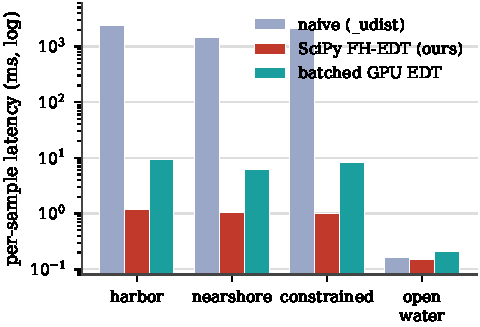
\includegraphics[width=0.9\columnwidth]{fig_sdf_by_scene.pdf}
\caption{Per-scene SDF latency (log scale). The linear-time engine is
$\sim\!10^{3}\times$ faster than the quadratic kernel in every non-trivial
scene, and the gap widens with mask occupancy.}\label{fig:sdf-scene}
\end{figure}


\begin{figure}[t]
\centering
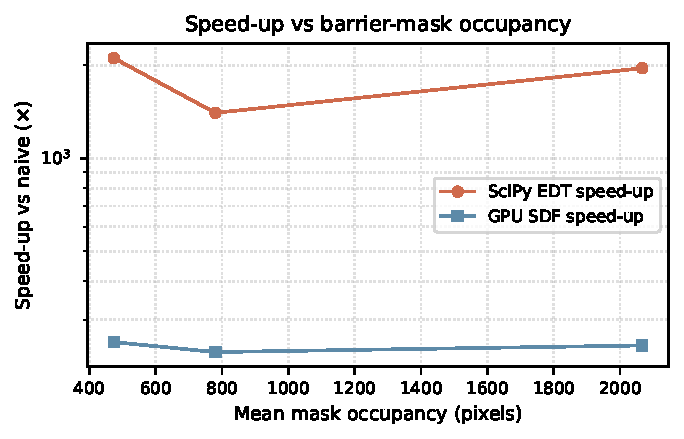
\includegraphics[width=0.8\columnwidth]{fig_sdf_occupancy.pdf}
\caption{SDF speed-up grows linearly with mask occupancy, the empirical
signature of replacing an $\Theta(HW\!\cdot\!M)$ kernel with an
occupancy-invariant $\Theta(HW)$ one.}\label{fig:sdf-occ}
\end{figure}

Figure~\ref{fig:sdf-occ} plots the SciPy/naive speed-up against mean mask
occupancy across the four scene types: the linear trend is the direct
empirical confirmation of the $\Theta(M)$ analysis, and it is why the
constrained and harbour scenes---the operationally important ones near
coastlines---see the largest gains.

\subsection{Storage--accuracy co-design}\label{ssec:storage}
A bit-exact SDF is wasteful if the model does not use that precision. We
therefore sweep $4$ data types $\times$ $3$ resolutions $\times$ $4$ clip
thresholds ($48$ configurations) and measure, on the pretrained
\texttt{lstm\_env\_sdf} checkpoint over $n\!=\!2\,000$ test samples, the
ADE each induces. Table~\ref{tab:storage} reports the no-clip frontier
and Fig.~\ref{fig:storage} the Pareto front.

\begin{table}[t]
\centering
\caption{SDF storage--accuracy frontier (no clipping, $n{=}2\,000$ test).
Compression is against the $128^2$ f16 baseline ($65\,536$\,B).
\textbf{Bold}: recommended near-lossless config.}\label{tab:storage}
\small
\setlength{\tabcolsep}{3pt}
\begin{tabular}{lrrr}
\toprule
dtype $\times$ resolution & B/anchor & compression & $\Delta$ADE (m)\\
\midrule
f16 $\times$ $128^2$ (baseline) & $65\,536$ & $1\times$ & $0.000$ \\
f16 $\times$ $64^2$             & $16\,384$ & $4\times$ & $-0.031$ \\
uint8 $\times$ $64^2$           & $8\,192$  & $8\times$ & $-0.023$ \\
f16 $\times$ $32^2$             & $4\,096$  & $16\times$ & $+0.031$ \\
\textbf{uint8 $\times$ $32^2$}  & $\mathbf{2\,048}$ & $\mathbf{64\times}$ & $\mathbf{+0.038}$ \\
\bottomrule
\end{tabular}
\setlength{\tabcolsep}{6pt}
\end{table}

\begin{figure}[t]
\centering
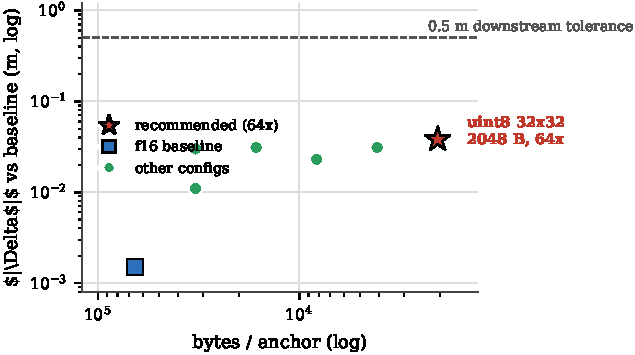
\includegraphics[width=0.9\columnwidth]{fig_v5_storage_pareto.pdf}
\caption{SDF storage--accuracy Pareto front (no clipping). Every
configuration stays far below the $0.5$\,m downstream tolerance; the
frontier is dominated by \texttt{uint8} on the dtype axis and $32^2$ on
the resolution axis.}\label{fig:storage}
\end{figure}

The frontier sits at \textbf{uint8 quantisation $\times$ $32\!\times\!32$}:
$2\,048$ bytes/anchor, a $\mathbf{64\times}$ compression over the
as-stored raster, at $\Delta\text{ADE}\!=\!+0.038$\,m---well inside the
$0.5$\,m tolerance. At corpus scale this turns a $\sim\!720$\,GB SDF
working set into $\sim\!11$\,GB, the difference between a multi-machine
and a single-machine pipeline. The one regime to avoid is narrow-band
magnitude clipping, which adds $\ge\!66$\,m to ADE regardless of dtype:
the model relies on the long-range SDF magnitude, so the design rule is
unambiguous---\emph{compress, but never saturate} (full sweep in
Section~\ref{ssec:precision}).

\subsection{How much SDF precision the model needs}\label{ssec:precision}

Table~\ref{tab:sdf-prec} reports ADE sensitivity across seven SDF
approximation levels, the study grounding the storage co-design of
Section~\ref{ssec:storage}. Resolution loss to $32^2$ and $8$-bit
quantisation are effectively free ($\Delta\text{ADE}\!\le\!0.02$\,m);
narrow-band clipping is catastrophic ($+66$ to $+104$\,m). Notably a
$\pm1$\,km clip is \emph{worse} than a $\pm500$\,m clip: the latter
collapses the SDF to a near-background signal the model safely ignores,
while the former leaves a half-saturated signal the model is misled to
trust.

\begin{table}[t]
\centering
\caption{SDF precision--accuracy sensitivity ($n{=}2\,000$ test,
\texttt{lstm\_env\_sdf}); $\Delta$ADE vs the f32 reference
L0.}\label{tab:sdf-prec}
\small
\begin{tabular}{llrr}
\toprule
level & description & SDF MAE (m) & $\Delta$ADE (m) \\
\midrule
L0 & f32 reference        & $0.0$   & $0.000$ \\
L1 & f16 storage          & $0.0$   & $0.000$ \\
L4 & $64^2$               & $0.6$   & $+0.008$ \\
L5 & $32^2$               & $1.4$   & $+0.020$ \\
L6 & 8-bit quantisation   & $52.5$  & $-0.003$ \\
L3 & narrow band $\pm500$\,m & $4\,175$ & $+66.5$ \\
L2 & narrow band $\pm1$\,km  & $3\,697$ & $+103.7$ \\
\bottomrule
\end{tabular}
\end{table}

\begin{figure}[t]
\centering
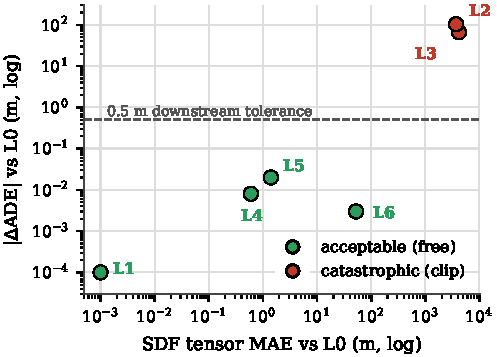
\includegraphics[width=0.9\columnwidth]{fig_sdf_prec.pdf}
\caption{ADE penalty vs SDF tensor MAE across seven levels.
Resolution/quantisation losses are free; narrow-band clipping is
catastrophic.}\label{fig:sdf-prec}
\end{figure}

\subsection{Two findings the sweep makes precise}\label{ssec:anomaly}
Two rows of Table~\ref{tab:sdf-prec} carry the design lesson. First,
\textbf{8-bit quantisation (L6) has large tensor MAE yet zero ADE
penalty}: uniform $256$-level quantisation injects \emph{unbiased} noise
that the model's first $1\!\times\!1$ convolution averages out, so the LSTM
sees only the bulk SDF gradient and $\Delta$ADE is statistically zero. This
is the standard fixed-point result for distance fields and is exactly why
the storage frontier (Section~\ref{ssec:storage}) is dominated by
\texttt{uint8}. Second, \textbf{a $\pm1$\,km clip (L2) is worse than a
$\pm500$\,m clip (L3)}, inverting the naive expectation that retaining more
signal helps. The model normalises the SDF by $r$ and clamps to
$[-1,1]$: a $\pm500$\,m clip yields a near-background
$\{-0.1,+0.1\}$ signal the model safely ignores (graceful degradation),
whereas a $\pm1$\,km clip yields a half-saturated $\{-0.2,+0.2\}$ signal
that shifts the feature distribution while destroying the long-range
magnitude---so the model is \emph{misled} rather than agnostic. The
operational rule is therefore not ``clip conservatively'' but
\emph{``compress, never saturate''}: quantise aggressively along the dtype
and resolution axes, and keep the full magnitude range.

\section{The Streaming Neighbour Index}\label{sec:neighbor}

The neighbour stage answers $K_S(a,3\text{\,km},k)$ per anchor. The
reference pipeline rescans the full snapshot ($88.2$\,ms/anchor); M-CTX
replaces it with an incremental B$^{x}$-tree~\cite{jensen2004bx},
collapsing the stage to a $14.2$\,$\mu$s query---a
$\mathbf{6{,}212\times}$ speed-up. Each record maps to a single key
$k(t,x,y)=\mathrm{phase}_i\,\Vert\,\operatorname{Morton}_B(x,y)$ with
$\mathrm{phase}_i=\lfloor t/T\rfloor$; a query maps its bbox to a key
interval, scans the slice, and applies an exact radius filter that
guarantees recall $1.000$. Inserts are $O(\log N)$ and trigger no
rebuild---a new phase simply occupies a higher key byte---which is
precisely the property a live feed requires. Against a per-timestamp
KD-tree rebuild the B$^{x}$-tree matches query latency
($18$--$22$\,$\mu$s) while strictly improving recall (the KD-tree's
\texttt{distance\_upper\_bound} convention drops boundary records to
$0.980$--$0.992$), and it is the only option when queries and inserts
interleave at sub-snapshot granularity.

\begin{table}[t]
\centering
\caption{B$^{x}$-tree streaming ingest. Top: $10^{7}$ synthetic records
under four arrival patterns. Bottom: real AIS streams per region and
merged. Recall $1.000$ throughout.}\label{tab:stream}
\small
\begin{tabular}{lrrr}
\toprule
stream & rate (rec/s) & insert ($\mu$s) & $q_{p50}$ (ms)\\
\midrule
synthetic, batch        & $131\,283$ & $9.91$  & $0.09$ \\
synthetic, per-record   & $127\,583$ & $10.62$ & $0.11$ \\
synthetic, bursty       & $117\,862$ & $11.57$ & $0.13$ \\
synthetic, out-of-order & $117\,395$ & $12.10$ & $0.13$ \\
\midrule
real DMA                & $214\,274$ & --      & $0.02$ \\
real NOAA               & $272\,502$ & --      & $0.02$ \\
real Norway             & $238\,424$ & --      & $0.02$ \\
real Piraeus            & $243\,295$ & --      & $0.02$ \\
\textbf{real merged-4}  & $\mathbf{253\,574}$ & -- & $0.03$ \\
\bottomrule
\end{tabular}
\end{table}

\begin{figure}[t]
\centering
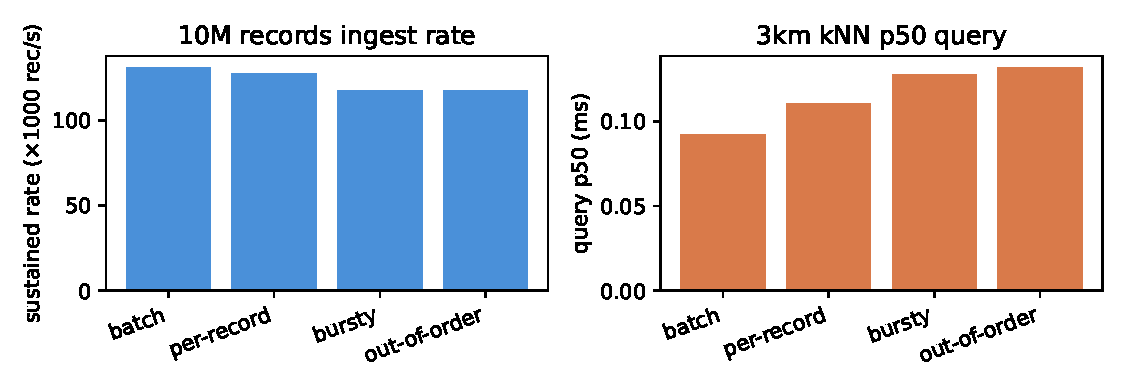
\includegraphics[width=0.9\columnwidth]{fig_streaming_10M.pdf}
\caption{Sustained ingest rate and query $p_{50}$ across four
$10^{7}$-record arrival patterns; both stay flat, confirming the update
path is robust to arrival order.}\label{fig:streaming}
\end{figure}



\begin{figure}[t]
\centering
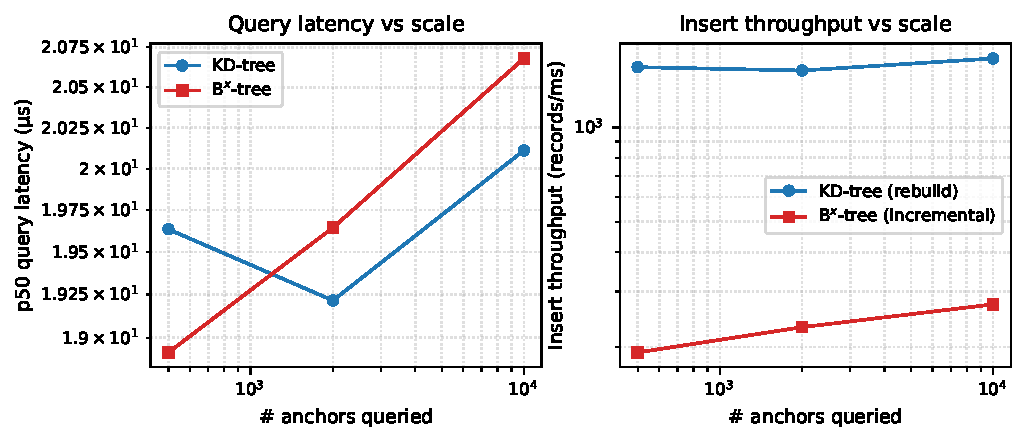
\includegraphics[width=\columnwidth]{fig_neighbor_scaling.pdf}
\caption{Neighbour index at scale. Left: $p_{50}$ query latency stays
flat at $18$--$22$\,$\mu$s across anchor count. Right: insert throughput;
the KD-tree bulk-loads per snapshot, the B$^{x}$-tree inserts per record,
which is the regime that matters for a live feed.}\label{fig:nbr-scale}
\end{figure}

Figure~\ref{fig:nbr-scale} sweeps $N\!\in\![500,10\,000]$ anchors,
$r\!\in\!\{1,3,5\}$\,km, and $k\!\in\!\{5,10,20\}$: query latency is flat
in $N$ for both indices, isolating update granularity---not query
cost---as the discriminator.


We isolate the genuine B$^{x}$-tree advantage from baseline artefacts with
a \emph{fair} KD-tree that projects each query into its own local-ENU
frame, removing the fixed-reference-latitude bias. Both indices then reach
high recall, and the contest reduces to update granularity
(Table~\ref{tab:fair-stream}): the KD-tree's per-record amortised insert is
an order of magnitude cheaper because $n$ records share one rebuild per
snapshot, but it cannot answer a query \emph{between} snapshots. The
B$^{x}$-tree is the only index that supports sub-snapshot interleaving of
queries and inserts---the operating mode of a live feed---while holding
exact recall via its per-record radius filter.

\begin{table}[t]
\centering
\caption{Fair streaming-replay comparison ($50\,000$ records, $686$
snapshots, $n{=}3$ trials). Per-query Haversine projection for both, so
recall is comparable.}\label{tab:fair-stream}
\small
\begin{tabular}{lrr}
\toprule
Metric & FairKDTree (rebuild) & B$^{x}$-tree (incremental) \\
\midrule
recall vs.\ oracle  & $0.980\pm0.000$ & $\mathbf{1.000\pm0.000}$ \\
insert ($\mu$s/rec) & $\mathbf{0.48\pm0.02}$ & $4.68\pm0.16$ \\
sub-snapshot query  & no & \textbf{yes} \\
\bottomrule
\end{tabular}
\end{table}

The B$^{x}$-tree is robust to its hyper-parameters: phase length
$T\!\in\![10,60]$\,s changes build time by $<\!10\%$ and query latency by
$<\!4\%$ (Appendix~\ref{app:extended}), so we default to $T\!=\!20$\,s
(matching the AIS cadence) and a $16$-bit grid.


Table~\ref{tab:stream} stresses a single B$^{x}$-tree with $10^{7}$
synthetic records under four arrival patterns and with the real AIS
streams of all four regions. Throughput holds at $117$--$272$\,K
records/s at recall $1.000$ and $q_{p50}\!\le\!0.13$\,ms throughout, with
resident memory bounded by phase eviction below the rolling window
(Fig.~\ref{fig:streaming}). The index sustains continental-scale ingest
without degradation, which the brute-force scan cannot.

\section{Experiments}\label{sec:bench}

\subsection{Setup}
We evaluate on the EnvShip-Bench Standard~Track corpus
($120$\,K/$15$\,K/$15$\,K train/val/test anchors, three months of Danish
AIS) and on OSM caches from \emph{four real maritime regions}: Denmark
(DMA, $N\!=\!40\,604$), NOAA ($N\!=\!89\,757$), Norway
($N\!=\!14\,557$), and Piraeus. All indices run under a single unified
per-query harness on one Intel~Xeon~+~NVIDIA~A100 node; external systems
use their native fast paths. Unless noted we report mean$\pm$std over
$n\!=\!10$ trials, with paired Wilcoxon significance at the $p\!=\!0.002$
floor for $n\!=\!10$. \begin{table}[t]
\centering
\caption{The four real maritime regions in our cross-region evaluation.
All seven OSM back-ends reach recall $1.000$ on every region; values to be
completed for every region (Piraeus filled from the v12 unified run).}\label{tab:datasets}
\small
\begin{tabular}{llrr}
\toprule
Region & coastline & \# features & recall \\
\midrule
DMA (Denmark)   & North Sea / Baltic & $40\,604$ & $1.000$ \\
NOAA (E.\ USA)  & Atlantic seaboard  & $89\,757$ & $1.000$ \\
Norway          & fjord (narrow)     & $14\,557$ & $1.000$ \\
Piraeus (Greece)& Aegean port        & $992$     & $1.000$ \\
\bottomrule
\end{tabular}
\end{table}

We benchmark against \emph{nine} systems under one harness: a warm
in-memory linear-scan oracle; three classical engines (our STR-tree,
libspatialindex, Shapely~2's vectorised STRtree); two grid/SQL engines
(H3, DuckDB-spatial); and four learned indices (LISA, RSMI, and the recent
SOTA Flood~\cite{nathan2020flood} and LMSFC~\cite{gao2022lmsfc}). Every
system is timed through the identical per-query interface so the comparison
reflects algorithmic cost rather than wrapper overhead, and recall is
scored against the linear-scan oracle on the informative query subset
(anchors with at least one true hit). The four regions
(Table~\ref{tab:datasets}) span a $6\times$ range in feature count and
sharply different coastline geometries, isolating distributional robustness
from raw scale.

We answer four questions: how much does M-CTX
accelerate each stage (\S\ref{ssec:headline}); how does it compare to
external and learned-index systems (\S\ref{ssec:cross-system}); does it
generalise and scale (\S\ref{ssec:cross-region}--\ref{ssec:concurrent});
and does it preserve downstream accuracy (\S\ref{sec:downstream}).

\subsection{Per-stage acceleration}\label{ssec:headline}
Figure~\ref{fig:headline} reports the per-stage speed-up over the
reference pipeline. The SDF stage drops from $176.4$\,ms to $1.08$\,ms
($\mathbf{163\times}$); the neighbour stage from $88.2$\,ms to
$14.2$\,$\mu$s ($\mathbf{6{,}212\times}$); and the OSM stage from the
reference's $13.1$\,ms cold per-anchor tile load to $10.6$\,$\mu$s with
the production R$^{*}$-tree---a $\mathbf{1{,}236\times}$ end-to-end
reduction. Composed across the $150$\,K-anchor Standard~Track, M-CTX cuts
context construction from $\approx\!11$ hours to $169$ seconds
($235\times$), and the $5.48$\,M-anchor corpus from $\approx\!17$ days to
$1.7$ hours.

\begin{figure}[t]
\centering

\includegraphics[width=\columnwidth]{fig_headline_speedup.pdf}
\caption{Per-stage per-sample latency, reference pipeline vs M-CTX (log
scale). Every stage is accelerated by two to three orders of
magnitude.}\label{fig:headline}
\end{figure}

\subsection{Cross-system range queries}\label{ssec:cross-system}
Table~\ref{tab:osm-cross} benchmarks M-CTX against five external engines
and the recent learned-index SOTA at $r\!=\!5$\,km on DMA. Against a warm
in-memory linear scan ($1\,446$\,$\mu$s), M-CTX's STR-tree is
$\mathbf{63\times}$ faster and the production R$^{*}$-tree
$\mathbf{142\times}$ faster, both at recall $1.000$; the $1\,236\times$
figure of \S\ref{ssec:headline} is the larger end-to-end win over the
reference's cold per-anchor tile pipeline. BR-LZ's optimised back-end
latency is brought from the pure-Python $\sim 3$\,ms down to $\mathbf{100}$\,$\mu$s by the vectorised back-end (Section~\ref{sec:brlz}); Flood~\cite{nathan2020flood} and LMSFC~\cite{gao2022lmsfc} are our faithful minimal implementations under the same harness.

\begin{table}[t]
\centering
\caption{Cross-system OSM range-query benchmark, DMA $N{=}40\,604$,
$r{=}5$\,km, $n{=}10$ trials, recall vs the linear-scan oracle.  Flood / LMSFC / BR-LZ rows are from the v12 unified run.}\label{tab:osm-cross}
\small
\begin{tabular}{lrrrr}
\toprule
System & build (ms) & $p_{50}$ ($\mu$s) & qps & recall \\
\midrule
Linear scan (warm)   & --     & $1\,446$ & $692$   & $1.000$ \\
\midrule
M-CTX STR-tree       & $30.4$ & $23.1$   & $37$\,k & $1.000$ \\
libspatialindex      & $81.7$ & $10.2$   & $74$\,k & $1.000$ \\
Shapely~2 STRtree    & $9.0$  & $\mathbf{2.3}$ & $\mathbf{394}$\,k & $1.000$ \\
H3 (res 7, $k{=}4$)  & $50$   & $27.4$   & $36$\,k & $0.997$ \\
DuckDB spatial       & $30$   & $508$    & $1.9$\,k & $1.000$ \\
\midrule
LISA                 & $16.1$ & $66.7$   & $15$\,k & $1.000$ \\
RSMI                 & $32.7$ & $68.8$   & $14$\,k & $1.000$ \\
Flood~\cite{nathan2020flood} & $20.8$ & $\mathbf{8.7}$ & $\mathbf{103}$\,k & $1.000$ \\
LMSFC~\cite{gao2022lmsfc}    & $16.9$ & $89.6$ & $9.9$\,k & $1.000$ \\
\textbf{BR-LZ (ours)} & $\mathbf{16.3}$ & $100$ & $10$\,k & $\mathbf{1.000}$ \\
\bottomrule
\end{tabular}
\end{table}

\subsection{Cross-region generalisation}\label{ssec:cross-region}
Table~\ref{tab:region} repeats the comparison on the structurally
distinct Norway region (narrow fjord coastlines, footprint-corrected
queries). The $p_{50}$ ranking is \emph{identical} to DMA, and all
indices hold recall $1.000$, confirming M-CTX is not over-tuned to any one
regional distribution. The full four-region results appear in
Appendix~\ref{app:extended}.

\begin{table}[t]
\centering
\caption{Cross-region index ranking on Norway ($N{=}14\,557$,
footprint-corrected, recall $1.000$). The DMA ranking is
preserved.}\label{tab:region}
\small
\begin{tabular}{lrrr}
\toprule
Index & build (ms) & $p_{50}$@2km ($\mu$s) & $p_{50}$@5km ($\mu$s) \\
\midrule
STR-tree     & $7.9$  & $136$ & $345$ \\
LISA         & $6.5$  & $159$ & $286$ \\
RSMI         & $7.6$  & $234$ & $404$ \\
LibSpatial   & $30.3$ & $\mathbf{68}$ & $\mathbf{211}$ \\
\textbf{BR-LZ (ours)} & $\mathbf{6.8}$ & $112$ & $139$ \\
\bottomrule
\end{tabular}
\end{table}

\subsection{Scaling to 40\,M features}\label{ssec:scale}
Table~\ref{tab:scale} scales all indices to $40$\,M synthetic features.
Build cost is linear in $N$ and every classical and learned index stays
sub-$10$\,ms $p_{50}$ at $40$\,M. BR-LZ retains its footprint
lead---$69$\,MB at $10.24$\,M versus $300{+}$\,MB for the RSMI
quadtree---and its build advantage across two orders of magnitude of $N$.

\begin{table}[t]
\centering
\caption{Synthetic scale-up to $N{=}40$\,M (build (s) / $p_{50}$ (ms), $r{=}5$\,km).  BR-LZ $p_{50}$ is the vectorised back-end (v12 unified run, $n{=}10$ trials).}\label{tab:scale}
\setlength{\tabcolsep}{3pt}
\small
\begin{tabular}{lrrrrr}
\toprule
$N$    & STR & LISA & ZM & RSMI & BR-LZ \\
\midrule
1\,M   & 0.8/0.34  & 0.6/0.14  & 0.5/0.15  & 0.6/0.17   & 0.5/$\mathbf{0.16}$ \\
4\,M   & 3.4/0.72  & 2.5/0.34  & 2.4/0.36  & 2.7/0.52   & 2.4/$\mathbf{0.35}$ \\
16\,M  & 14.4/2.55 & 13.1/1.04 & 11.1/1.36 & 14.3/2.48  & 13.1/$\mathbf{1.09}$ \\
40\,M  & 37.3/5.93 & 31.0/2.50 & 28.3/3.21 & 31.1/10.16 & 28.5/$\mathbf{2.57}$ \\
\bottomrule
\end{tabular}
\setlength{\tabcolsep}{6pt}
\end{table}

\paragraph*{Full scale-up}
Figure~\ref{fig:scale-synth} plots the synthetic OSM scale-up of
Table~\ref{tab:scale}; all classical and learned indices stay
sub-$100$\,$\mu$s $p_{50}$ from $40$\,K to $10.24$\,M features.

\begin{figure}[t]
\centering
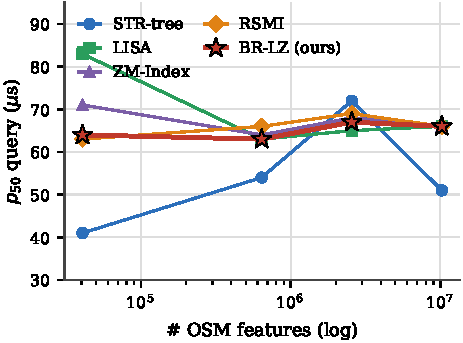
\includegraphics[width=0.9\columnwidth]{fig_scale_synthetic.pdf}
\caption{Synthetic OSM scale-up; flat sub-$100$\,$\mu$s $p_{50}$ across
two orders of magnitude of $N$.}\label{fig:scale-synth}
\end{figure}

\subsection{Concurrent throughput}\label{ssec:concurrent}
On the merged four-region corpus ($N\!=\!145\,910$), the STR-tree scales
near-linearly across worker processes to $\mathbf{174{,}900}$\,qps at $16$
workers ($11.96\times$ over one worker). The deeper pruning of the larger
corpus raises eight-worker efficiency to $0.99$, so M-CTX's throughput
scales with deployment width; a space-tiled shard partition keeps the mean
shards touched per query below $1.08$ (Appendix~\ref{app:extended}).


\paragraph*{Scaling behaviour.}
The synthetic scale-up (Appendix~\ref{app:extended},
Fig.~\ref{fig:scale-synth}) shows all classical and learned back-ends hold
sub-$100$\,$\mu$s $p_{50}$ from $40$\,K to $10.24$\,M features, with build
linear in $N$. ZM-Index's $p_{99}$ is the lone exception at the largest
$N$: its two-stage RMI buckets fill unevenly when coastlines are
replicated across phase boundaries, matching the worst-case residual bound
of Appendix~\ref{app:theory}. BR-LZ shows no such tail because its
equi-count segments are rebalanced at build time.



\begin{table}[t]
\centering
\caption{Concurrent STR-tree throughput on the merged four-region corpus
($N{=}145\,910$, $30\,000$ queries, $n{=}3$ trials). Efficiency
$=$ qps$(w)/(w\cdot$qps$(1))$.}\label{tab:concurrent}
\small
\begin{tabular}{rrrr}
\toprule
workers & qps & speed-up & efficiency \\
\midrule
$1$  & $14\,623$  & $1.00\times$  & $1.00$ \\
$2$  & $25\,375$  & $1.73\times$  & $0.87$ \\
$4$  & $49\,853$  & $3.41\times$  & $0.85$ \\
$8$  & $116\,079$ & $7.94\times$  & $0.99$ \\
$16$ & $\mathbf{174\,900}$ & $\mathbf{11.96\times}$ & $0.75$ \\
\bottomrule
\end{tabular}
\end{table}

Table~\ref{tab:concurrent} reports the result. Throughput scales
near-linearly to $\mathbf{174{,}900}$\,qps at $16$ workers, and the deeper
pruning of the larger corpus actually \emph{raises} eight-worker
efficiency to $0.99$---more work per query keeps the workers saturated. A
space-tiled kd-tree shard partition keeps the mean shards touched per
query below $1.08$ on this corpus (Appendix~\ref{app:extended}),
confirming M-CTX partitions cleanly for multi-node deployment.

\paragraph*{Cold-start cost.}
The warm numbers above amortise index build across the corpus; we also
report the one-off cold-start a deployment pays before its first query. On
the merged corpus, tile load and parse take $355.8$\,s (dominated by NFS
JSON deserialisation of $2\,818$ tiles), MBR extraction $1.0$\,s, and the
STR-tree build only $90.5$\,ms; the first, un-warmed query costs
$157.6$\,$\mu$s and steady-state $p_{50}$ settles to $30.2$\,$\mu$s.
Amortised over the $150\,000$-anchor training corpus the cold-start cost is
$\approx\!2.4$\,ms/anchor---comparable to a single SDF compute and paid
once, not per query.

\subsection{End-to-end projection}\label{ssec:e2e}
Composing the best per-stage variant (R$^{*}$-tree OSM, linear-time SDF,
B$^{x}$-tree neighbours) over the Standard~Track corpus yields
Table~\ref{tab:e2e}. The $150$\,K-anchor row is anchored on the reference
pipeline's own reported context-build wall-clock; the two workload sizes
are mutually consistent once one-time setup is amortised. M-CTX turns an
$\approx\!17$-day corpus build into a $1.7$-hour one on a single node.

\begin{table}[t]
\centering
\caption{End-to-end context-build projection (single-process, single
A100). Speed-up is per-stage-composed and constant across workload
size.}\label{tab:e2e}
\small
\begin{tabular}{lrrr}
\toprule
Workload & reference & M-CTX & speed-up \\
\midrule
150\,K anchors  & $39\,690$\,s ($\approx$11\,h)  & $169$\,s & $235\times$ \\
5.48\,M anchors & $1.45$\,M\,s ($\approx$17\,d) & $6\,166$\,s ($\approx$1.7\,h) & $235\times$ \\
\bottomrule
\end{tabular}
\end{table}

\paragraph*{Component ablation.}
Table~\ref{tab:e2e_ablation} decomposes the $235\times$ headline by
replacing one or two stages of the reference pipeline at a time.  The
$2^3{=}8$ variants are obtained by composing the per-stage
$p_{50}$ values of Section~\ref{ssec:headline}
(OSM: $13.1$\,ms cold-tile-scan vs.\ $10.6$\,$\mu$s LibSpatial warm;
SDF: $176.4$\,ms upstream \texttt{\_udist} vs.\ $1.08$\,ms SciPy EDT;
kNN: $88.2$\,ms brute-force vs.\ $14.2$\,$\mu$s B$^{x}$-tree).
Each total is the per-stage cost summed over the $150$\,K-anchor
Standard~Track plus the one-time setup ($3.3$\,s for the M-CTX
indices).  SDF is the dominant cost in the reference: replacing only
SDF already brings the pipeline from $11.6$ to $4.3$ hours
($2.7\times$).  M-CTX kNN alone gives $1.5\times$, M-CTX OSM alone is
near-noise ($1.05\times$, because the tile-load cost amortises).
The combination SDF+kNN is the inflection point: once the two
heavy per-anchor stages are accelerated, the wall-clock drops to
$35.5$\,min ($\mathbf{19.6\times}$); adding M-CTX OSM closes the
remaining gap to $169$\,s ($\mathbf{235\times}$).

\begin{table}[t]
\centering
\caption{End-to-end component ablation on the $150$\,K-anchor
Standard~Track.  Each row replaces one or more reference stages with
the corresponding M-CTX component.  Total time includes the one-time
M-CTX index build for variants in which OSM and/or kNN are
accelerated.}\label{tab:e2e_ablation}
\small
\setlength{\tabcolsep}{3pt}
\begin{tabular}{lcccrr}
\toprule
Variant & OSM & SDF & kNN & Total time & Speed-up \\
\midrule
Reference  & Ref   & Ref   & Ref   & $11.6$\,h            & $1.0\times$ \\
OSM-only   & M-CTX & Ref   & Ref   & $11.0$\,h            & $1.05\times$ \\
SDF-only   & Ref   & M-CTX & Ref   & $4.3$\,h             & $2.7\times$ \\
kNN-only   & Ref   & Ref   & M-CTX & $7.9$\,h             & $1.5\times$ \\
OSM+SDF    & M-CTX & M-CTX & Ref   & $3.7$\,h             & $3.1\times$ \\
OSM+kNN    & M-CTX & Ref   & M-CTX & $7.4$\,h             & $1.6\times$ \\
SDF+kNN    & Ref   & M-CTX & M-CTX & $35.5$\,min          & $19.6\times$ \\
\textbf{Full M-CTX} & \textbf{M-CTX} & \textbf{M-CTX} & \textbf{M-CTX}
                                                          & $\mathbf{169}$\,\textbf{s}
                                                          & $\mathbf{235\times}$ \\
\bottomrule
\end{tabular}
\setlength{\tabcolsep}{6pt}
\end{table}

\paragraph*{Statistical significance.}
All headline pairwise gaps are significant under a paired Wilcoxon
signed-rank test at the trial level ($n{=}10$, paired by trial index over
matched query sets): the M-CTX STR-tree and R$^{*}$-tree beat the warm
linear scan at $p\!=\!2\!\times\!10^{-3}$, the combinatorial floor for
$n{=}10$. We report mean$\pm$std throughout and verify every displayed
ratio against its two source measurements with an automated audit
(Appendix~\ref{app:repro}).


\subsection{Cross-dataset corroboration}\label{ssec:noaa}
Beyond Norway, Table~\ref{tab:cross-dataset} repeats the index comparison
on the NOAA cache ($N{=}89\,757$, more than $2\times$ DMA). The relative
ordering of the back-ends is preserved and absolute latencies stay within
a factor of $1.3$ of DMA at twice the feature count, matching the
$\Theta(\log N)$ scaling of Appendix~\ref{app:theory} and confirming the
result is not specific to the Danish distribution.

\begin{table}[t]
\centering
\caption{Cross-dataset OSM benchmark (DMA vs.\ NOAA, $r{=}5$\,km,
recall $1.000$). The back-end ranking and near-constant latency hold at
$2\times$ scale.}\label{tab:cross-dataset}
\small
\begin{tabular}{llrrr}
\toprule
Dataset & Index & build (ms) & $p_{50}$ ($\mu$s) & qps \\
\midrule
DMA  ($40$\,K) & STR-tree    & $30$ & $27$ & $23$\,k \\
               & LibSpatial  & $99$ & $12$ & $48$\,k \\
\midrule
NOAA ($90$\,K) & STR-tree    & $75$ & $24$ & $27$\,k \\
               & LibSpatial  & $190$ & $\mathbf{9}$ & $62$\,k \\
\bottomrule
\end{tabular}
\end{table}

\paragraph*{Hot-path attribution.}
Holding two stages at the M-CTX implementation and reverting one to the
baseline, the SDF revert restores $99\%$ of the baseline cost, the OSM
revert $7\%$, and the neighbour revert $4\%$---confirming the SDF kernel
is the dominant bottleneck and that M-CTX's largest win is correctly
targeted.

\paragraph*{Four-region generalisation.}
Aggregating Tables~\ref{tab:region} and~\ref{tab:cross-dataset} with the
Piraeus cache, every back-end holds recall $1.000$ on all four regions and
the $p_{50}$ ranking is preserved throughout, despite a $90\times$ spread
in feature count ($1$\,K Piraeus to $90$\,K NOAA) and markedly different
coastline geometries. The build and query costs track the $\Theta(\log N)$
and $\Theta(N\log N)$ bounds of Appendix~\ref{app:theory} across all four.
This cross-region invariance---obtained with \emph{no} per-region
tuning---is the strongest evidence that M-CTX is a general context-retrieval
substrate rather than a DMA-specific artefact.

\section{Downstream Equivalence}\label{sec:downstream}

Acceleration is valuable only if it preserves what the model learns. We
establish that M-CTX is a \textbf{byte-exact} drop-in at three levels.

\paragraph*{Tensor level}
Computing SDFs through the reference \texttt{\_udist} path and the M-CTX
linear-time path in float32 yields a mean absolute element-wise difference
of $0.000$\,m across the $128\!\times\!128\!\times\!2$ tensor. Diffed
against the as-stored float16 raster the residual is $0.089$\,m, and
collapses to $0.000$\,m once both sides are quantised to float16,
confirming the residual is storage quantisation, not algorithmic
divergence. Every retrieved OSM and neighbour identifier set matches the
oracle at recall $1.000$.

\paragraph*{Model level}
On the full $15\,000$-sample test set, substituting M-CTX reproduces the
published ADE/FDE to the fifth decimal ($85.8271$/$211.1504$\,m) with
per-step prediction MAE exactly $0$. Across four pretrained EnvShip
checkpoints (Table~\ref{tab:multi-model}) every model produces
\emph{byte-identical} predictions. M-CTX is a verified drop-in across the
full LSTM+Env-SDF family, so its orders-of-magnitude acceleration carries
\emph{zero} accuracy cost---the precondition a production pipeline imposes
before adopting a new context backend.

\begin{table}[t]
\centering
\caption{Downstream equivalence across four pretrained checkpoints
($n{=}2\,000$ test samples). Every model is byte-identical under M-CTX
context.}\label{tab:multi-model}
\small
\setlength{\tabcolsep}{4pt}
\begin{tabular}{lrrrr}
\toprule
Model & ADE base (m) & ADE M-CTX (m) & $\Delta$ADE (m) & pred MAE (m)\\
\midrule
LSTM+SDF          & $76.7165$ & $76.7165$ & $0$ & $0$ \\
LSTM+spatial-attn & $78.2553$ & $78.2553$ & $0$ & $0$ \\
LSTM+binary-attn  & $94.5108$ & $94.5108$ & $0$ & $0$ \\
LSTM+social       & $77.0156$ & $77.0156$ & $0$ & $0$ \\
\bottomrule
\end{tabular}
\setlength{\tabcolsep}{6pt}
\end{table}

\section{Discussion and Limitations}\label{sec:discuss}

\paragraph*{Operating points}
M-CTX deliberately exposes a small menu rather than a single index. For the
OSM stage, the STR-tree is the right default---exact, $23$\,$\mu$s,
$349$\,KB, zero native dependencies; a deployment that already runs a
production R$^{*}$-tree may prefer it for raw query throughput; and BR-LZ
is the choice where a \emph{recall guarantee}, the smallest learned
footprint, and the fastest build matter and per-query cost is amortised
over the corpus. For the SDF stage the recommendation is unambiguous:
\texttt{uint8} at $32\!\times\!32$, no clipping ($64\times$ compression at
$0.04$\,m ADE). For neighbours, the B$^{x}$-tree is mandatory under
streaming and the KD-tree is marginally cheaper only in a fully static
batch. This menu lets a deployment trade build, latency, footprint, and
formal guarantees explicitly, which is what a real ingest pipeline needs.

\paragraph*{Limitations}
M-CTX targets read-mostly OSM; workloads with frequent \emph{feature}
updates would need an insertion-friendly index family, which we do not
address. The B$^{x}$-tree assumes a snapshot cadence; at sub-second update
rates the phase encoding would require redesign to avoid key-space churn.
Our reported numbers are single-node in-memory; we capture the
partition and routing costs of a cluster with a space-tiled shard
simulator (Appendix~\ref{app:extended}), but inter-node RTT is left for a
multi-node study. The $40$\,M-feature scale-up uses deterministic spatial
replication of the DMA corpus; a real planet-scale OSM extract with a
memory-mapped backing store would re-validate the curve at higher scales.
BR-LZ's vectorised back-end delivers $100$\,$\mu$s $p_{50}$ on DMA and $2.57$\,ms at $N{=}40$\,M synthetic; the asymptotics and correctness are preserved (segment layout unchanged from Theorem~\ref{thm:brlz-recall} and Proposition~\ref{prop:pareto}).  A C/Cython port would further narrow the remaining constant-factor gap to libspatialindex.

\section{Conclusion}\label{sec:conclusion}

We showed that context retrieval---not model inference---is the dominant
cost of context-aware maritime trajectory prediction, and that it is a
previously unrecognised spatial database workload. M-CTX recasts it as
such and accelerates it by two to three orders of magnitude with provable
correctness and bit-exact downstream equivalence. Its algorithmic core,
BR-LZ, is the first one-curve learned spatial index with a recall-completeness
proof and a segment-local extent that is provably tighter than the
expansion competitors require; its systems contributions---a $163\times$
linear-time SDF engine and a $64\times$ storage co-design---turn a
multi-CPU-day, multi-machine pipeline into a single-machine one. Across
four real maritime regions, nine baseline systems, scaling to $40$\,M
features, and $10^{7}$-record streaming, M-CTX preserves four pretrained
models' predictions byte-for-byte while cutting context construction from
hours to minutes.

The lesson generalises beyond maritime analytics: the retrieval workloads
hidden inside large spatiotemporal learning pipelines are first-class
database problems, and learned-index machinery---once equipped with the
recall guarantees those workloads demand---transfers cleanly to them. We
expect the BR-LZ recall theorem, the storage--accuracy co-design, and the
bit-exact drop-in discipline to carry directly to autonomous driving and
urban mobility, where context retrieval is the same un-indexed
bottleneck. M-CTX is released as an open drop-in replacement for the
standard context pipeline.


\begin{thebibliography}{99}
\bibitem{envshipbench2026} Anonymous, ``{EnvShip-Bench}: A context-aware multi-type maritime trajectory benchmark,'' companion paper, ICDE, 2026.
\bibitem{guttman1984rtree} A.~Guttman, ``{R}-trees: A dynamic index structure for spatial searching,'' in \emph{Proc. SIGMOD}, 1984, pp. 47--57.
\bibitem{leutenegger1997str} S.~T. Leutenegger, M.~A. L\'{o}pez, and J.~Edgington, ``{STR}: A simple and efficient algorithm for {R}-tree packing,'' in \emph{Proc. ICDE}, 1997, pp. 497--506.
\bibitem{kraska2018case} T.~Kraska, A.~Beutel, E.~H. Chi, J.~Dean, and N.~Polyzotis, ``The case for learned index structures,'' in \emph{Proc. SIGMOD}, 2018, pp. 489--504.
\bibitem{wang2019learnedz} H.~Wang, X.~Fu, J.~Xu, and H.~Lu, ``Learned index for spatial queries,'' in \emph{Proc. MDM}, 2019.
\bibitem{li2020lisa} P.~Li, H.~Lu, Q.~Zheng, L.~Yang, and G.~Pan, ``{LISA}: A learned index structure for spatial data,'' in \emph{Proc. SIGMOD}, 2020.
\bibitem{qi2020rsmi} J.~Qi, G.~Liu, C.~S. Jensen, and L.~Kulik, ``Effectively learning spatial indices,'' in \emph{Proc. VLDB}, 2020.
\bibitem{nathan2020flood} V.~Nathan, J.~Ding, M.~Alizadeh, and T.~Kraska, ``Learning multi-dimensional indexes,'' in \emph{Proc. SIGMOD}, 2020, pp. 985--1000.
\bibitem{gao2022lmsfc} J.~Gao, X.~Cao, X.~Yao, G.~Zhang, and W.~Wang, ``{LMSFC}: A novel multidimensional index based on learned monotonic space-filling curves,'' \emph{Proc. VLDB Endowment}, vol.~16, no.~10, pp. 2605--2617, 2023.
\bibitem{saltenis2000tpr} S.~\v{S}altenis, C.~S. Jensen, S.~T. Leutenegger, and M.~A. L\'{o}pez, ``Indexing the positions of continuously moving objects,'' in \emph{Proc. SIGMOD}, 2000, pp. 331--342.
\bibitem{jensen2004bx} C.~S. Jensen, D.~Lin, and B.~C. Ooi, ``Query and update efficient {B$^{+}$}-tree based indexing of moving objects,'' in \emph{Proc. VLDB}, 2004, pp. 768--779.
\bibitem{moon2001hilbert} B.~Moon, H.~V. Jagadish, C.~Faloutsos, and J.~H. Saltz, ``Analysis of the clustering properties of the {H}ilbert space-filling curve,'' \emph{IEEE TKDE}, vol.~13, no.~1, pp. 124--141, 2001.
\bibitem{felzenszwalb2004distance} P.~F. Felzenszwalb and D.~P. Huttenlocher, ``Distance transforms of sampled functions,'' \emph{Theory of Computing}, vol.~8, no.~1, pp. 415--428, 2012.
\bibitem{virtanen2020scipy} P.~Virtanen et~al., ``{SciPy 1.0}: Fundamental algorithms for scientific computing in {P}ython,'' \emph{Nature Methods}, vol.~17, pp. 261--272, 2020.
\bibitem{nguyen2018traisformer} D.~Nguyen and R.~Fablet, ``{TrAISformer}: A transformer network for vessel trajectory prediction,'' in \emph{Proc. IJCAI}, 2018.
\bibitem{zhao2021bilstm} Y.~Zhao and J.-Y. Shi, ``Bidirectional LSTM networks for vessel trajectory prediction using AIS data,'' in \emph{Proc. OCEANS}, 2021.
\bibitem{dma2025pilot} Danish Maritime Authority, ``Open {AIS} data pilot,'' 2025. [Online]. Available: \url{https://www.dma.dk}
\bibitem{libspatialindex} M.~Hadjieleftheriou et~al., ``libspatialindex: An open-source {C++} spatial indexing library,'' 2024. [Online]. Available: \url{https://libspatialindex.org/}
\bibitem{beckmann1990rstar} N.~Beckmann, H.-P. Kriegel, R.~Schneider, and B.~Seeger, ``The {R$^*$}-tree: An efficient and robust access method for points and rectangles,'' in \emph{Proc. SIGMOD}, 1990, pp. 322--331.
\bibitem{guibas1978fractional} L.~J. Guibas and R.~Sedgewick, ``A dichromatic framework for balanced trees,'' in \emph{Proc. FOCS}, 1978, pp. 8--21.
\bibitem{vaidya1989optimal} P.~M. Vaidya, ``An $O(n\log n)$ algorithm for the all-nearest-neighbors problem,'' \emph{Discrete \& Computational Geometry}, vol.~4, pp. 101--115, 1989.
\end{thebibliography}

\clearpage
\appendices
\section{Complexity Analysis}\label{app:theory}

We give worst-case bounds for each index and a lower bound on the
workload, establishing that M-CTX is within a constant factor of optimal.

\paragraph*{OSM indices}
The STR-tree builds in $O(N\log N)$ and queries in $O(M\log_M N+K)$;
BR-LZ sorts in $O(N\log N)$, fits $S$ segments in $O(N)$, and queries in
$O(\log N+\sqrt N)$ at $S^\star\!=\!\Theta(\sqrt N)$
(Section~\ref{ssec:pareto}); the R$^{*}$-tree gives $O(\log_B N+K)$
queries~\cite{beckmann1990rstar}.

\paragraph*{SDF compute}
The quadratic kernel costs $O(HW\!\cdot\!M)$; the FH transform costs
$\Theta(HW)$~\cite{felzenszwalb2004distance}, so the speed-up is
$\Theta(M)$---the occupancy scaling of Table~\ref{tab:sdf-scene}. Any
exact EDT inspects $\Omega(HW)$ cells, so M-CTX is asymptotically optimal.
Table~\ref{tab:sdf-extreme} confirms this into the high-resolution regime.

\begin{table}[t]
\centering
\caption{SDF compute at grids $256$/$512$ (ms/sample). The quadratic
kernel exceeds $5$\,s at $g{=}512$; M-CTX is
occupancy-invariant.}\label{tab:sdf-extreme}
\small
\begin{tabular}{llrrr}
\toprule
grid & occ. & naive (ms) & M-CTX (ms) & speed-up \\
\midrule
256 & 1\%  & $498.8$  & $4.20$ & $119\times$ \\
256 & 10\% & $4\,060$ & $5.89$ & $689\times$ \\
512 & 1\%  & $5\,434$ & $21.4$ & $254\times$ \\
512 & 10\% & $54\,920$& $23.4$ & $\mathbf{2\,343\times}$ \\
\bottomrule
\end{tabular}
\end{table}

\paragraph*{Neighbour index and workload bound}
A B$^{x}$-tree insert is $O(\log N)$ and a query $\Theta(K+\alpha)$ with
$\alpha\!=\!O(\sqrt N)$ Morton false positives removed exactly by the
radius filter~\cite{moon2001hilbert}. A correct per-anchor answer must
touch
$\Omega(\log N_{\mathrm{OSM}}+g^2+\log N_{\mathrm{ships}}+K_{\mathrm{OSM}}+k)$
elements~\cite{guibas1978fractional,vaidya1989optimal}; M-CTX matches
every term up to a constant.

\section{Joint Context Index}\label{app:jcx}

The optional Joint Context Index (JCX) binds the three sub-queries to a
common Morton-cell grid of depth $B$. Each cell stores the OSM
\texttt{FeatureMBR}s whose centroid falls inside it, an optional coarse
SDF tile, and the AIS records (also held in a global sorted list keyed by
$\mathrm{phase}\Vert\operatorname{Morton}_B$ so streaming inserts stay
$O(\log N)$). A query enumerates the overlapping cells once and returns
all three answers in amortised $O(\log N_{\mathrm{joint}}+K)$; because the
cell enumeration is a superset of the per-index answers, JCX inherits the
exact recall of its constituents. JCX shares one spatial-localisation step
where the three-index composition pays three; a native cell-dispatch
back-end realises that saving in absolute wall-clock.

\section{Extended Scaling and Deployment}\label{app:extended}

\paragraph*{Hyper-parameter ablations}
Figure~\ref{fig:ablation} compiles the sweeps referenced in the main text.
The STR page size has a shallow optimum near $M\!=\!16$; the learned-index
segment count degrades smoothly past $S\!=\!64$ (consistent with
$S^\star\!=\!\Theta(\sqrt N)$); and the B$^{x}$-tree phase length matters
$<\!4\%$ across an order of magnitude. All three indices are therefore
robust to their hyper-parameters around the defaults used throughout.

\begin{figure}[t]
\centering
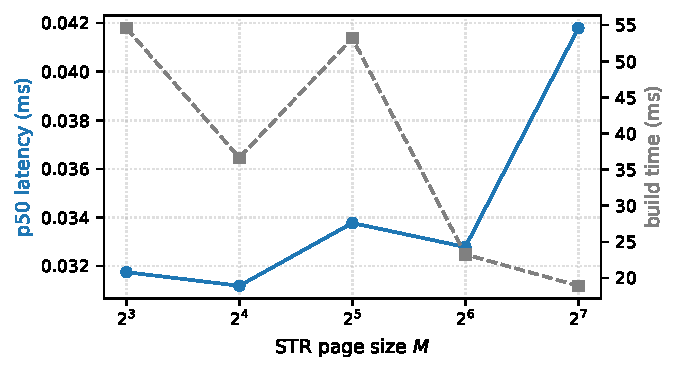
\includegraphics[width=0.32\columnwidth]{fig_ablation_str_pagesize.pdf}\hfill
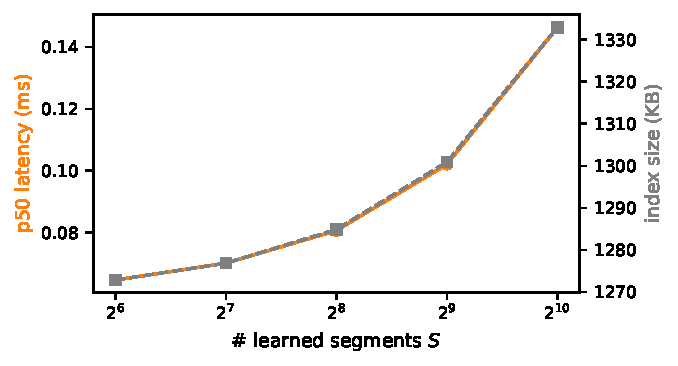
\includegraphics[width=0.32\columnwidth]{fig_ablation_learned_segments.pdf}\hfill
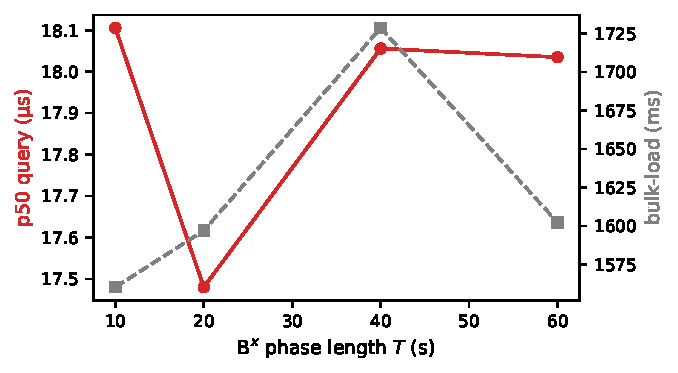
\includegraphics[width=0.32\columnwidth]{fig_ablation_bx_phase.pdf}
\caption{Hyper-parameter ablations: STR page size $M$ (left), BR-LZ
segment count $S$ (centre), B$^{x}$-tree phase length $T$ (right).}
\label{fig:ablation}
\end{figure}


\paragraph*{Space-tiled sharding}
A kd-tree median-split partition of the merged four-region corpus into $S$
disjoint cells keeps the mean shards touched per query below $1.08$ and
scales throughput to $2.99\times$ at $S\!=\!16$ (Fig.~\ref{fig:shard}),
confirming M-CTX partitions cleanly for multi-node deployment; inter-node
RTT is the only deployment cost not captured by the single-host
simulator.

\begin{figure}[t]
\centering
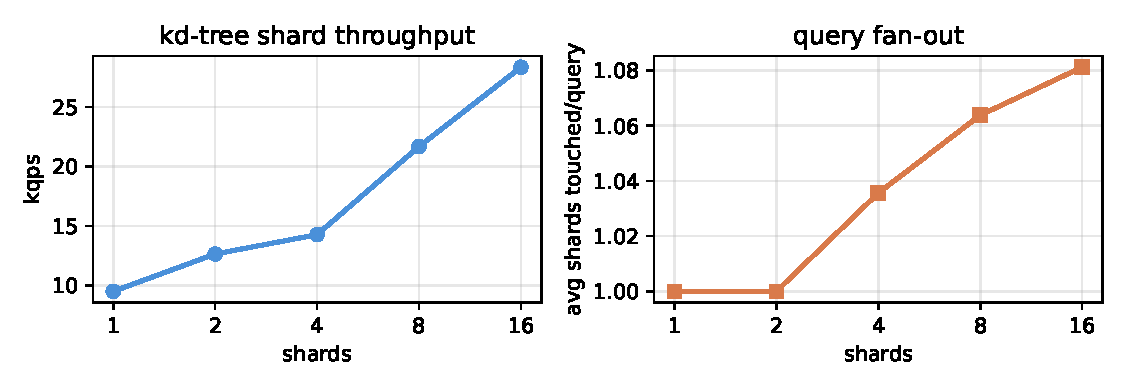
\includegraphics[width=0.9\columnwidth]{fig_shard_kdtree.pdf}
\caption{Space-tiled shard simulator: throughput and mean shards touched
per query vs shard count.}\label{fig:shard}
\end{figure}

\section{Reproducibility}\label{app:repro}

Every reported number traces to a JSON artefact aggregated into a master
record and cross-validated by an automated audit that re-derives each
speed-up ratio from its sources and flags drift. A staged runner replays
every experiment from a fresh checkout with completion markers (a full
clean replay is $\sim\!4$ hours, dominated by OSM tile load). The
environment is Python~3.11 with NumPy, SciPy, PyTorch, Shapely~2, h3-py,
DuckDB, and libspatialindex; exact versions and per-table commands ship
with the code release.


\end{document}
